% How and why the system is structured that way

\chapter{Methodology}
\label{chap:method}

\section{Research Approach}
This thesis follows a design- and implementation-oriented methodology aimed at developing and evaluating a privacy-preserving extension for Android applications that use Custom Tabs (CTs) and Trusted Web Activities (TWAs).
The main research goal is to prevent HyTrack's cross-app tracking attack \cite{USENIX:Wessels:2025} by addressing the underlying weaknesses identified in \autoref{sec:hytrack-weaknesses}, while adhering to the design goals defined by Wessels et al. in \autoref{sec:hytrack-goals}.
Unlike previously discussed mitigation strategies such as Browser State Partitioning or Forced User Interaction (\autoref{sec:hytrack-mitigations}), the proposed approach aims to maintain usability and compatibility while providing strong privacy guarantees.

To address this gap, this work develops and evaluates a privacy-preserving extension for Android applications that use Custom Tabs (CTs) and Trusted Web Activities (TWAs).
The proposed framework prevents HyTrack’s cross-app tracking attack \cite{USENIX:Wessels:2025} by eliminating the architectural weaknesses identified in \autoref{sec:hytrack-weaknesses}, while adhering to the design goals of usability, compatibility, and controlled access to shared state \autoref{sec:hytrack-goals}.

The core idea is to encapsulate cookie access within fine-grained capability tokens, created and validated by the browser according to a developer-defined policy.
Depending on the policy configuration, cookies are stored either in a shared global jar or in app-specific storage, analogous to the Partitioned attribute in CHIPS \cite{googlechips}.
This design prevents unauthorized cross-app tracking while preserving legitimate use cases such as Single Sign-On and session continuity.
Because the system operates solely at the app–browser boundary, it maintains full compatibility with existing web platform features and requires no changes to the browser UI.

\section{Capability Tokens}
Against the natural feature of capabilities being delegatable, we need to bind them to the app identity to prevent cross-app tracking by simple token reuse.
Therefore, we include the apps identity in the capability tokens, so that the browser can verify that the token is only used by the app it was issued to.
Similar to JWTs~\cite{rfc7519}, our tokens are signed to identify tampering attemtps.
Due to the Thread Model assumptions {\autoref{sec:threat_model}}, we additionally need to encrypt the tokens, so that a malicious third-party library embedded in the app cannot read the token contents and echo them back to its web server to circumvent the mitigation.
In conclusion, we design our capability tokens to be identity-bound and cryptographically protected data structures that encapsulate cookie information and metadata, enabling fine-grained access control between Android apps and the browser.

% -----------------------Explain Methodology Flow Diagram Here ---------------------------
\section{Lifecycle and Flow}
\begin{figure}[h!]
  \centering
  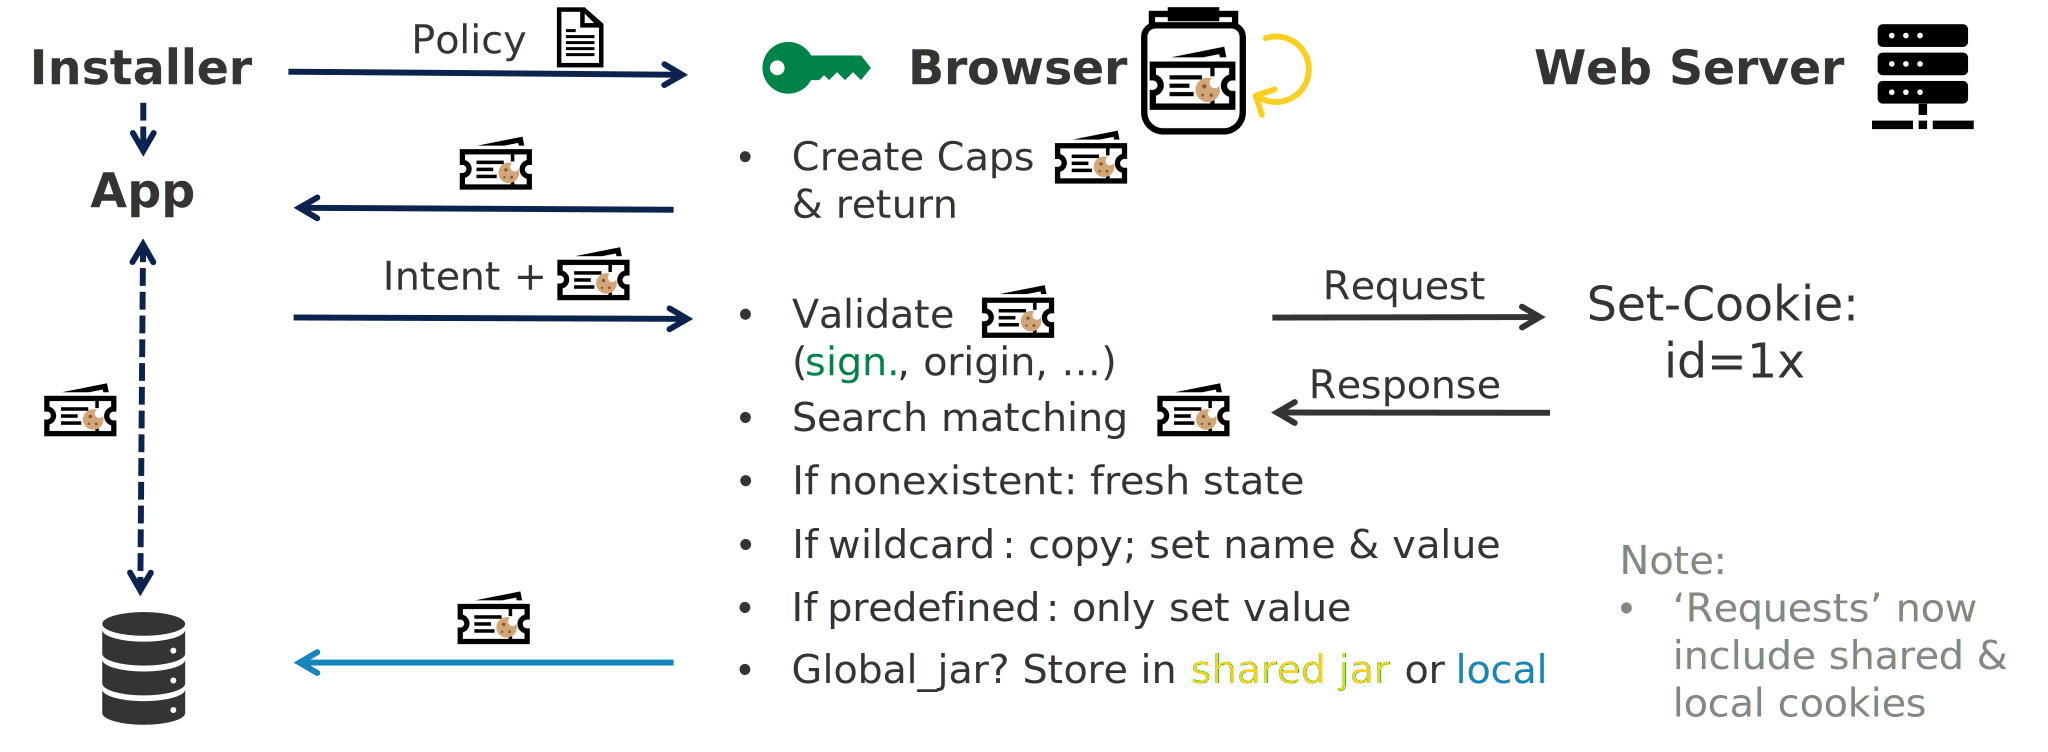
\includegraphics[width=0.9\textwidth]{ByeTrack_Flow.pdf}
  \caption{High-level overview of the Byetrack flow between installer, app, browser, and web servers.}
  \label{fig:byetrack_overview}
\end{figure}

To achieve this, a prototype framework named Byetrack was designed, implemented, and evaluated on Android.
The framework consists of three main components: a custom installer for policy extraction, a helper library for application integration, and modifications to the Mozilla Fenix browser and its underlying GeckoView engine to enforce cookie isolation via capability tokens.

\subsection{Developer Policy}
Developers define a JSON policy that specifies which domains may share browser state and, optionally, which cookies are expected from each domain.
This allows granular control beyond simple trusted/untrusted domain distinctions -- for example, isolating third-party cookies while permitting integration with a developer's own authentication domain or SSO provider.
If no policy is provided, the browser falls back to ambient mode, where all cookies are stored in the shared jar for backwards compatibility.

\subsection{Capability Initialization}

\begin{figure}[h!]
  \centering
  \includegraphics[width=0.9\textwidth]{InitTokenFlowChart.drawio.pdf}
  \caption{Flow of capability initialization during app installation.}
  \label{fig:initialization_flow}
\end{figure}

During app installation, the installer extracts and transmits the policy to the browser.
The browser validates and sanitizes the policy to ensure minimal privilege, removing conflicting or ambiguous entries.  

From the sanitized policy, the browser generates capability tokens as follows:
\begin{itemize}
  \item For predefined cookie entries, the browser creates corresponding predefined capability tokens.
  \item For domain-level entries, the browser issues wildcard capabilities, marking them as global or private based on the policy.
  \item If no policy is provided, a single ambient capability is issued, reverting to the default shared-cookie behavior.
\end{itemize}

Each token is signed and encrypted before being sent to the app, which stores wildcard and final tokens in private storage for later use.  
When the app is updated, the installer retransmits the policy so that the browser can reissue capabilities consistent with the new app version.

\subsection{App–Browser Interaction}

\begin{figure}[h!]
  \centering
  \includegraphics[width=0.9\textwidth]{byetrack_Flow_Flowchart_colored.pdf}
  \caption{Flow of app–browser-server interaction regarding cookie isolation during URL launches.}
  \label{fig:app_browser_interaction}
\end{figure}

When an app opens a URL through a Custom Tab (CT) or Trusted Web Activity (TWA), the stored wildcard and (initially empty) final tokens are attached to the intent that launches the browser.
Upon receipt, the browser decrypts and validates each token by checking its signature, package name, version number, and target domain.
Invalid tokens are discarded.

The browser then uses the valid capabilities to:
\begin{enumerate}[label=\arabic*.]
  \item Determine how to store cookies received from the web server.
  \item Construct cookie headers for outgoing requests.
\end{enumerate}

\paragraph{Cookie Reception.}  
For every received cookie, the browser applies the following logic (in order of priority):
\begin{enumerate}[label=\arabic*.]
  \item If the token is ambient, the cookie is stored in the global jar (default behavior).
  \item If a private predefined capability matches the cookie name, the cookie value is filled in and returned to the app for local storage.
  \item If a private wildcard capability exists, the cookie is filled in accordingly and returned to the app.
  \item If a global predefined capability matches, the cookie is stored in the shared jar.
  \item If a global wildcard capability exists, any cookie from the corresponding domain is stored in the shared jar.
  \item If no capability matches, the cookie is discarded.
\end{enumerate}

\paragraph{Cookie Transmission.}  
When constructing requests, the browser merges cookies derived from the app's valid final tokens with those from its global jar, ensuring that each request accurately reflects both app-specific and shared state according to the developer policy.

% ---------------------------------------------------------------------------

\subsection{Utility Interfaces}
To improve transparency and developer control, the browser exposes limited utility functions that allow the app to:
\begin{enumerate}[label=\arabic*)]
  \item Retrieve the names of cookies encapsulated in final capabilities.
  \item Read their corresponding values.
  \item Write or update cookie values.  
\end{enumerate}
Access to these utilities is strictly controlled through capability rights: read operations require read rights, and modifications require write rights.

\section{Design Advantages} % move this to another section?
Beyond preventing cross-app tracking, Byetrack offers several key benefits:
\begin{enumerate}[label=B\arabic*)]
  \item \textbf{Fine-Grained Control:} Developers can precisely specify which cookies are shared or isolated.
  \item \textbf{Stateless Browser Design:} The browser remains stateless with respect to app-specific data, as apps retain and transmit their own tokens.
  \item \textbf{No Web Server Changes:} Web servers operate unmodified—the browser transparently enforces the capability model.
  \item \textbf{Backwards Compatibility:} Apps without a policy fall back to the standard shared cookie behavior, ensuring compatibility with existing systems.
\end{enumerate}

\section{Alternative Design Considerations}
An alternative architecture would delegate capability generation to the installer rather than the browser.  
This would simplify the browser's responsibilities to enforcement only, reducing its complexity and eliminating installer–browser communication for each app.
It would also solve the bootstrapping problem of generating the initial capabiltities the current design faces: if an app is installed on a device, the installer notifies the browser of the new app and its policy so the browser can generate capabilities accordingly.
If this browser is not installed yet, the app cannot receive capabilities until the browser is installed and the app is reinstalled or updated.
Having the installer generate capabilities would allow the app to receive them immediately upon installation, regardless of the browser's presence and whether it even supports the framework or not.
However, it would require shared cryptographic secrets between the installer and browser, thereby enlarging the trusted computing base and attack surface.  
For this and simplicitly reasons, the proof-of-concept implementation designates the browser as the sole trusted component for capability generation and enforcement and assumes the browser is present before app installation.


%\subsection{Token Fields}
%The following fields form the basis:
%
%\begin{itemize}
%  \item \textbf{Cookie Name and Value:} Contain the actual cookie data managed by the browser.
%  \item \textbf{Signature:} Ensures the capability was issued by the browser and has not been modified.
%  \item \textbf{Package Name:} Identifies the app that owns the capability.  
%    This prevents implicit delegation—without it, a receiving app could reuse capabilities issued to another app.
%  \item \textbf{Domain:} Specifies the target web server.  
%    The browser enforces that cookies are only valid for this domain, preventing malicious libraries from reusing capabilities to store untrusted cookies in the global jar.
%  \item \textbf{App Version Number:} Allows the browser to detect outdated tokens after app updates.  
%    Whenever the app is updated, the installer retransmits the policy so the browser can issue new capabilities consistent with the new version.
%  \item \textbf{Rights:} Define the permitted actions—reading, writing, or both—on cookie data.  
%    These rights prevent tracking libraries from exploiting browser access to extract or misuse capability contents.
%  \item \textbf{Global Jar Flag:} Indicates whether the cookie belongs to the shared global jar or to the app-specific isolated jar.
%\end{itemize}
%
%\subsection{Capability Types}
%We distinguish between \texttt{final}, \texttt{wildcard}, and \texttt{ambient} capabilities.
%
%\begin{itemize}
%  \item \textbf{Final Capabilities:} Fully specified tokens containing explicit cookie names and values.  
%    They represent concrete cookie instances and are used directly for cookie enforcement.
%  \item \textbf{Wildcard Capabilities:} Partially specified tokens that omit cookie names or values.  
%    They serve as templates from which final tokens are derived once cookies are received from a web server.
%  \item \textbf{Ambient Capabilities:} Represent the browser’s default behavior—storing all cookies in the shared global jar.  
%    These act as fallbacks when no explicit policy is provided and offer no privacy guarantees.
%\end{itemize}
